\section{Space complexity}
\label{sec:space_complexity}

\begin{frame}
	\frametitle{Space complexity}
	\framesubtitle{Anywhere in space and time}
	\begin{center}
		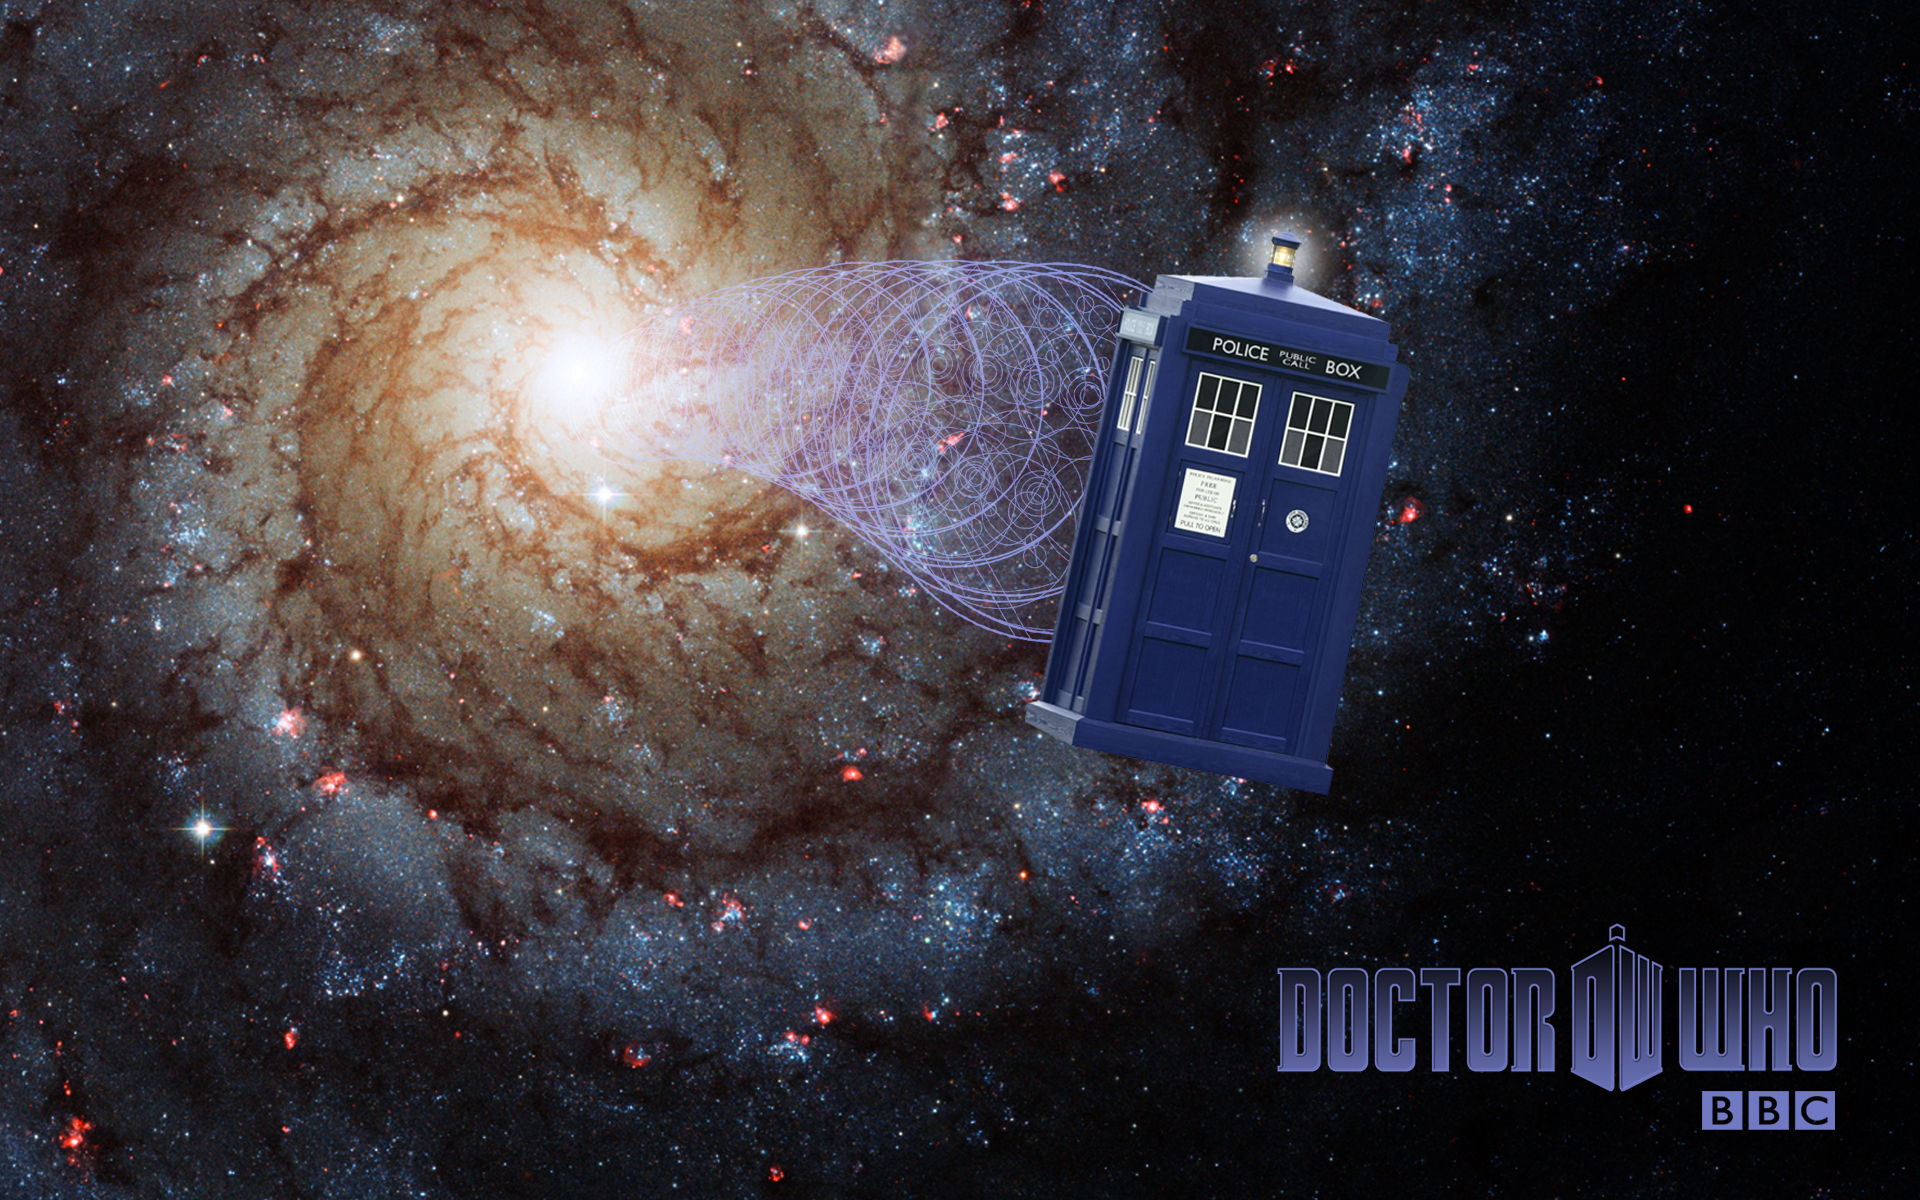
\includegraphics[width=0.73\textwidth]{figures/tardis.jpg}\\
		\hspace*{15pt}\hbox{\scriptsize Image By:\thinspace{\itshape anna\_thetical}}
		%https://www.flickr.com/photos/anna_thetical/4147623095
	\end{center}
\end{frame}

\begin{frame}
	\frametitle{Space complexity}
	\begin{itemize}
		\item So far we have only looked at the required \alert{time} of a function.
		\item What about the required \alert{space}?
			\pause
		\item Just like time, space is a \alert{finite} resource.	
		\item So it is important to be able to set bounds on the usage.
	\end{itemize}
	\pause
	\begin{questionblock}{Difference?}
		Is there any difference in how time and space are used by functions?
	\end{questionblock}
	\pause
	\begin{answerblock}{Recycling}
		Yes! Space can be reused, whereas time cannot.
	\end{answerblock}
\end{frame}

\begin{frame}
	\frametitle{A first example}
	\framesubtitle{Creating a list}
	
	\begin{columns}
		\column{0.455\textwidth}
			\lstinputlisting{code/comprehension-complexity.py}
		\column{0.455\textwidth}
		\pause
		\begin{questionblock}{Space}
			What is the \alert{space} complexity of this list comprehension?
			\begin{enumerate}[A.]
				\item $\Theta(1)$
				\item $\Theta(n)$ 
				\item $\Theta(n^2)$
				\item I don't know.
			\end{enumerate}
		\end{questionblock}
	\end{columns}
	\pause
	\begin{answerblock}{Linear time}
		We have $n$ integers, each requiring some constant amount of space $c$. Thus $S(n) = cn$, so $\Theta(n)$ space is
		required.
	\end{answerblock}
\end{frame}

\begin{frame}
	\frametitle{Memory in a computer}
	\framesubtitle{The following slides are based on slides originally created by Robbert Krebbers}
\begin{center}
	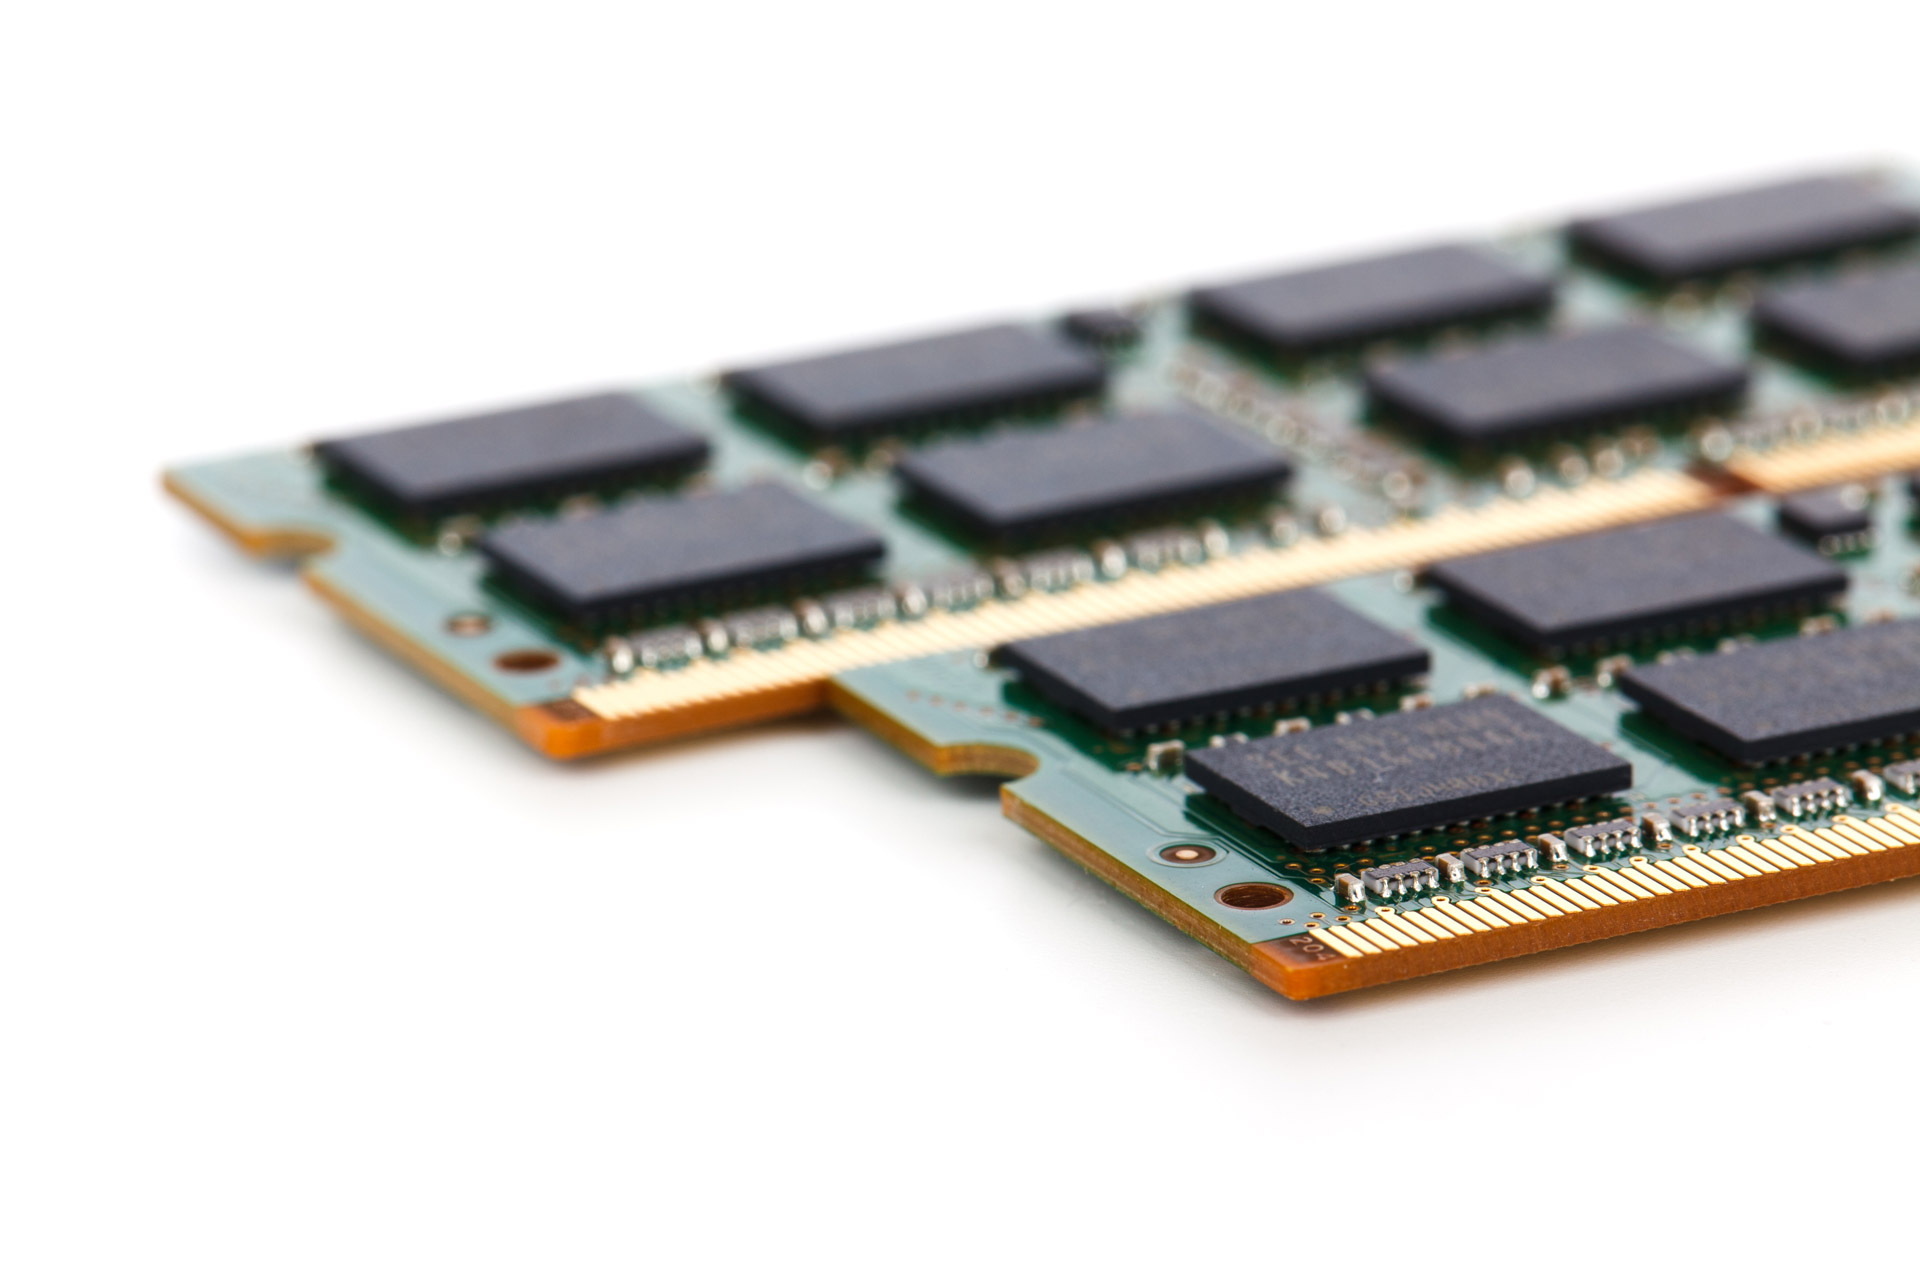
\includegraphics[width=0.70\textwidth]{figures/ram.jpg}\\
	\hspace*{15pt}\hbox{\scriptsize Image By:\thinspace{\itshape Petr Kratochvil}}
	%https://www.publicdomainpictures.net/en/view-image.php?image=18285&picture=ram-modules
\end{center}
\end{frame}


\begin{frame}
	\frametitle{Function calls}
	\framesubtitle{Based on a slide by Robbert Krebbers}
	\begin{columns}
		\column{0.455\textwidth}
		\small
		\textbf{When a function is called:}
		\begin{itemize}
			\item A \emph{stack frame} is \emph{added} to memory.
			\item The stack frame contains:
				\begin{itemize}
					\item The function arguments
					\item The local variables
					\item The \emph{return address} to track the statement that called the function
				\end{itemize}
		\end{itemize}

		\medskip
		\textbf{When a function returns:}
		\begin{itemize}
			\item The \emph{stack frame} is \emph{removed}.
			\item Control returns to the \emph{return address}.
		\end{itemize}
		\column{0.455\textwidth}

		\begin{tikzpicture}[
			node distance=0.2em,
			stackframe/.style={draw=black,
			text width=4.5em,minimum height=3em,text centered,font=\small},
			]
			\node[stackframe,fill=green!10] (main) {
				stack frame for \lstinline|main|
			};
			\node[stackframe,above=of main,fill=green!20] (f) {
				stack frame for \lstinline|f|
			};
			\node[stackframe,above=of f,fill=green!30] (g) {
				stack frame for \lstinline|g|
			};

			\node[stackframe,left=0.5em of g,yshift=5em,fill=green!40] (push) {stack frame for \lstinline|h|};
			\node[stackframe,right=0.5em of g,yshift=5em,fill=green!30] (pop) {stack frame for \lstinline|g|};

			\draw[->,thick] (push) edge[out=0,in=90] node[left,yshift=-1.5em] {add} ($(g.north)+(-1em,0)$);
			\draw[<-,thick] (pop) edge[out=180,in=90] node[right,yshift=-1.5em] {remove} ($(g.north)+(1em,0)$);

		\end{tikzpicture}
	\end{columns}

	\pause
	\begin{columns}[t]
		\column{0.755\textwidth}

		\begin{questionblock}{The same function?}
			Can there be multiple frames for the same function on the stack?
		\end{questionblock}
		\pause
		\column{0.255\textwidth}
		\begin{answerblock}{Yes!}
			Recursion!
		\end{answerblock}
	\end{columns}
\end{frame}

\begin{frame}[fragile]{The call stack in action}
	\framesubtitle{Based on a slide by Robbert Krebbers}
\begin{minipage}[t]{0.5\textwidth}
\textbf{Let us call \lstinline|foo(3)|}:

\medskip
\begin{lstlisting}[linebackgroundcolor={%
  \btLstHL<1>{}%
  \btLstHL<2>{5-8}%
  \btLstHL<3>{6-8}%
  \btLstHL<5>{7-8}%
  \btLstHL<7>{8-8}%
  \btLstHL<4,6>{2}%
}]
def bar(n: int) -> int:
  return n;

def foo(n: int) -> int:
	res = 8
	res += bar(n-1) 
	res += bar(n-2) 
	return res
\end{lstlisting}

\medskip
\onslide<2->{
\textbf{When a function is called:}
\begin{itemize}
\item A \emph{stack frame} is \emph{added} to the stack
\item Containing the function arguments, local variables, and the \emph{return address}
\end{itemize}}
\end{minipage}
\hfill
\begin{minipage}[t]{0.48\textwidth}
\textbf{Stack:}

\smallskip
\begin{tikzpicture}[
  node distance=0.2em,
  stackframe/.style={font=\small,draw=structure,thick,fill=structure!0.1,text width=8em},
	every label/.style={right,font=\scriptsize\tt},
]
\onslide<2->{\node[stackframe,label=right:foo(3),onslide=<2-3>{draw=alert},onslide=<5>{draw=alert},onslide=<7>{draw=alert}] (foo) {
  \texttt{n} = 3 \\
  \texttt{res} = \only<2-4>{8}\only<5-6>{10}\only<7->{11} \\
  \texttt{return}=\emph{main}
};}

\onslide<4>{\node[stackframe,label=right:bar(2),above=of foo,onslide=<4>{draw=alert}] (fac2) {
  \texttt{n} = 2 \\
  \texttt{return}=line~6
};}

\onslide<6>{\node[stackframe,label=right:bar(1),above=of foo,onslide=<6>{draw=alert}] (fac1b) {
  \texttt{n} = 1 \\
  \texttt{return}=line~7
};}

\invisible{\node[stackframe,label=right:factorial(2),above=of fac1b,onslide=<6>{draw=alert}] (fac2b) {
  \texttt{n} = 1 \\
  \texttt{n} = 1 \\
  \texttt{n} = 1 \\
  \texttt{return}=line~7
};}
\end{tikzpicture}

\medskip
\onslide<4->{
\textbf{When a function returns:}
\begin{itemize}
\item The \emph{stack frame} is \emph{removed}
\item Control returns to the \emph{return address}
\end{itemize}}
\end{minipage}
\end{frame}

\begin{frame}
	\frametitle{A long story short}
	
	Observations:
	\begin{itemize}
		\item Calling a function takes space!
		\item This is important when dealing with recursive functions (which we will discuss after the break).
		\item All of the parameters are stored in this bit of space as well.
	\end{itemize}
	\pause
	\begin{questionblock}{What about lists?}
		Does this mean that the ``stack frame'' for \texttt{baz(my\_list)} requires $O(n)$ space?
	\end{questionblock}
	\pause
	\begin{answerblock}{Nope}
		No! We pass a \textit{reference} instead of a copy. We tell \texttt{baz} where the list is so that it can
		access (or change!) it. Thus this call still requires only $O(1)$ space.\\

		{\scriptsize
		See this excellent StackOverflow post explaining this in more detail if you are interested:
	\url{https://stackoverflow.com/a/986145}.}
	\end{answerblock}
\end{frame}

\begin{frame}
	\frametitle{A second example}
	\framesubtitle{Using a list}
	
	\begin{columns}
		\column{0.455\textwidth}
		\lstinputlisting{code/big-oh-example.py}
		\column{0.455\textwidth}
		\pause
		\begin{questionblock}{Space}
			What is the space complexity of the function \texttt{maya}?
			\begin{enumerate}[A.]
				\item $\Theta(1)$
				\item $\Theta(n)$ 
				\item $\Theta(n^2)$
				\item I don't know.
			\end{enumerate}
		\end{questionblock}
	\end{columns}
	\pause
	\begin{answerblock}{Quadratic space}
		We create a list of $n^2$ items, so we need $\Theta(n^2)$ space. We could say $S(n) = c_0 + c_1n^2$, where $c_0$ is
		for the stack frame, \texttt{s}, \texttt{i} and \texttt{j}. $c_1$ is for \texttt{x}.
	\end{answerblock}
\end{frame}

\begin{frame}
	\frametitle{A second example - modified}
	\framesubtitle{Doing without the list}
	
	\begin{columns}
		\column{0.455\textwidth}
		\lstinputlisting{code/big-oh-example-v2.py}
		\column{0.455\textwidth}
		\pause
		\begin{questionblock}{Space}
			What is the space complexity of the function \texttt{mia}?
			\begin{enumerate}[A.]
				\item $\Theta(1)$
				\item $\Theta(n)$ 
				\item $\Theta(n^2)$
				\item I don't know.
			\end{enumerate}
		\end{questionblock}
	\end{columns}
	\pause
	\begin{answerblock}{Constant space}
		We now only require to store the variable \texttt{s} and call the function \texttt{range}. Both of these require
		constant space, so $S(n) = c_0$ is $\Theta(1)$.
	\end{answerblock}
\end{frame}

\begin{frame}
	\frametitle{A final example - modified}
	\framesubtitle{Using a list from a parameter}
	
	\begin{columns}
		\column{0.455\textwidth}
		\lstinputlisting{code/big-oh-example-v3.py}
		\column{0.455\textwidth}
		\pause
		\begin{questionblock}{Space}
			What is the space complexity of the function \texttt{sum}?
			\begin{enumerate}[A.]
				\item $\Theta(1)$
				\item $\Theta(n)$ 
				\item $\Theta(n^2)$
				\item I don't know.
			\end{enumerate}
		\end{questionblock}
	\end{columns}
	\pause
	\begin{answerblock}{Constant space}
		Remember that a list that is passed as input, is a \textit{reference} and does not take space!
	\end{answerblock}
	\pause
		\begin{block}{Observation}
			Had input contributed to the space complexity, there would be no sub-linear space complexities!	
		\end{block}	
\end{frame}

\begin{frame}
	\frametitle{Relations between time and space?}
	\begin{questionblock}{It's all (a) relative (dimension)}
		Given that a function \texttt{foo} uses $\Theta(n)$ space, what, if anything, can we conclude about the amount of
		time $T(n)$ \texttt{foo} requires?
		\begin{enumerate}[A.]
			\item $T(n)$ is $\Omega(n)$
			\item $T(n)$ is $\Theta(n)$
			\item $T(n)$ is $O(n)$
			\item We cannot conclude anything.
			\item I don't know
		\end{enumerate}
	\end{questionblock}
		\pause
		\begin{answerblock}{A nice lower bound}
			Claiming all of this memory (space) requires time! So we need $\Omega(n)$ time to execute \texttt{foo}!
		\end{answerblock}
\end{frame}
